\documentclass[tikz, border=8pt]{standalone}
\usepackage[T1]{fontenc}
\usepackage{tgpagella}
\usepackage{mathpazo}
\usepackage{tikz}
\usepackage{amsmath}
\usepackage{amssymb}
\usepackage{xcolor}
\usepackage{fontawesome5}
\usetikzlibrary{positioning, arrows.meta, shapes.geometric, fit, backgrounds, calc}

% ----------------------------------------------------------------
% Inline palette -- mirrors figures/_palette.tex (AGENTS.md rule 1).
% Kept inline so this figure compiles stand-alone regardless of
% TEXINPUTS, matching figures/architecture.tex.
% ----------------------------------------------------------------
\definecolor{cAudio}{HTML}{F5EFE3}
\definecolor{cEnc}{HTML}{DDE9EC}
\definecolor{cEncB}{HTML}{2D8294}
\definecolor{cAdp}{HTML}{F0DFC9}
\definecolor{cAdpB}{HTML}{B07849}
\definecolor{cLLM}{HTML}{F4E6D5}
\definecolor{cLLMB}{HTML}{A0763C}
\definecolor{cPrompt}{HTML}{F1ECE3}
\definecolor{cPromptB}{HTML}{8E7A55}
\definecolor{cTok}{HTML}{E5EEF0}
\definecolor{cTokB}{HTML}{5E8090}
\definecolor{cBound}{HTML}{ECDFD3}
\definecolor{cBoundB}{HTML}{9C7558}

\tikzset{
  module/.style    ={draw, rounded corners=3pt, align=center,
                     font=\small, line width=0.7pt,
                     minimum width=3.4cm, minimum height=0.9cm},
  audio/.style     ={module, fill=cAudio, draw=black!35},
  encoder/.style   ={module, fill=cEnc, draw=cEncB,
                     minimum width=10.0cm, minimum height=1.1cm},
  adapter/.style   ={module, fill=cAdp, draw=cAdpB},
  promptbox/.style ={module, fill=cPrompt, draw=cPromptB},
  boundbox/.style  ={module, fill=cBound, draw=cBoundB},
  outbox/.style    ={module, fill=white, draw=black!50,
                     minimum width=8.6cm, minimum height=1.0cm,
                     font=\small},
  dashedmod/.style ={module, fill=cTok!35, draw=cTokB, dashed,
                     line width=0.6pt, font=\small},
  flow/.style      ={-Stealth, line width=0.7pt, draw=black!70},
  dashedflow/.style={flow, dashed, draw=black!55},
  edgelabel/.style ={font=\scriptsize, text=black!55,
                     fill=white, inner sep=1pt},
  resourcebox/.style = {audio, minimum width=3.6cm, minimum height=1.2cm,
                        align=center},
}

\begin{document}
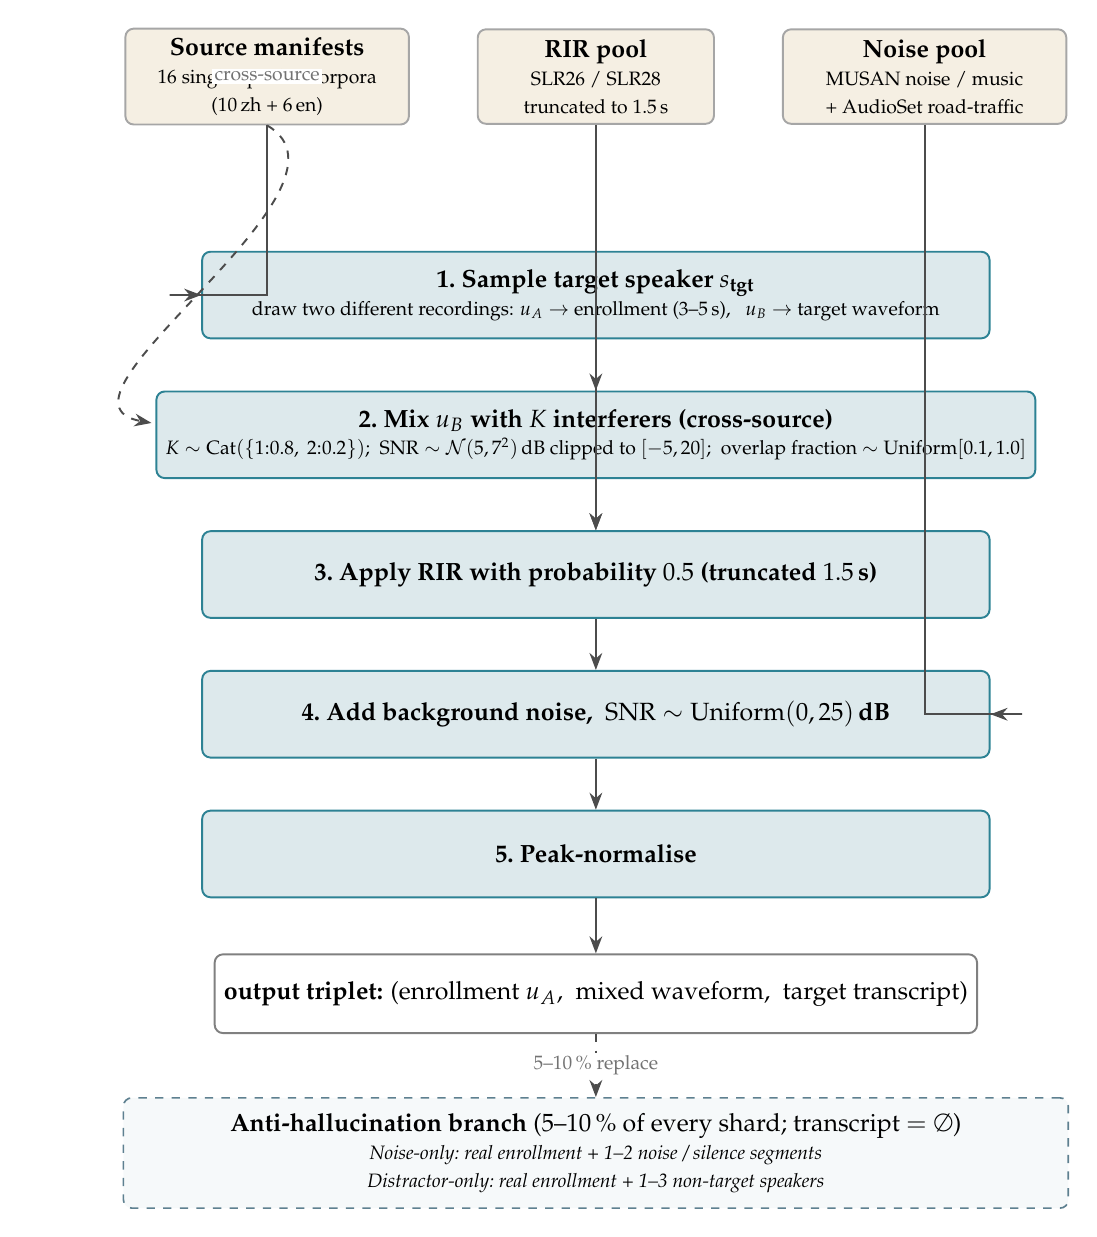
\begin{tikzpicture}[node distance=0.65cm and 0.85cm]

  % ============================================================
  % RESOURCE ROW (top): 3 side-data pools
  % ============================================================
  \node[resourcebox] (srcman) {%
    \textbf{Source manifests}\\[-1pt]
    {\scriptsize 16 single-speaker corpora}\\[-1pt]
    {\scriptsize (10\,zh + 6\,en)}};

  \node[resourcebox, right=of srcman, minimum width=3.0cm] (rirpool) {%
    \textbf{RIR pool}\\[-1pt]
    {\scriptsize SLR26 / SLR28}\\[-1pt]
    {\scriptsize truncated to $1.5\,$s}};

  \node[resourcebox, right=of rirpool] (noisepool) {%
    \textbf{Noise pool}\\[-1pt]
    {\scriptsize MUSAN noise / music}\\[-1pt]
    {\scriptsize + AudioSet road-traffic}};

  % ============================================================
  % MAIN PIPELINE (center, vertical 5 steps)
  % ============================================================
  \node[encoder, below=1.6cm of rirpool.south] (step1) {%
    \textbf{1.~Sample target speaker $s_\text{tgt}$}\\[-1pt]
    {\scriptsize draw two different recordings:
     $u_A$ $\to$ enrollment (3--5\,s),~~
     $u_B$ $\to$ target waveform}};

  \node[encoder, below=of step1] (step2) {%
    \textbf{2.~Mix $u_B$ with $K$ interferers (cross-source)}\\[-1pt]
    {\scriptsize $K \sim \mathrm{Cat}(\{1{:}0.8,~2{:}0.2\})$;~
     $\mathrm{SNR}\sim\mathcal{N}(5,7^2)\,$dB clipped to $[-5,20]$;~
     overlap fraction $\sim\mathrm{Uniform}[0.1,1.0]$}};

  \node[encoder, below=of step2] (step3) {%
    \textbf{3.~Apply RIR with probability $0.5$ (truncated $1.5\,$s)}};

  \node[encoder, below=of step3] (step4) {%
    \textbf{4.~Add background noise,~
            $\mathrm{SNR}\sim\mathrm{Uniform}(0,25)\,$dB}};

  \node[encoder, below=of step4] (step5) {%
    \textbf{5.~Peak-normalise}};

  \node[outbox, below=0.7cm of step5] (output) {%
    \textbf{output triplet:} (enrollment $u_A$,~ mixed waveform,~ target transcript)};

  % ============================================================
  % ANTI-HALLUCINATION BRANCH (bottom, dashed)
  % ============================================================
  \node[dashedmod, below=0.8cm of output,
        minimum width=12.0cm, minimum height=1.4cm,
        align=center] (negbox) {%
    \textbf{Anti-hallucination branch} (5--10\,\% of every shard;
    transcript $=\emptyset$)\\[-1pt]
    {\scriptsize\itshape Noise-only:~real enrollment + 1--2 noise / silence segments}\\[-1pt]
    {\scriptsize\itshape Distractor-only:~real enrollment + 1--3 non-target speakers}};

  % ============================================================
  % ARROWS
  % ============================================================
  % Main pipeline downward
  \draw[flow] (step1) -- (step2);
  \draw[flow] (step2) -- (step3);
  \draw[flow] (step3) -- (step4);
  \draw[flow] (step4) -- (step5);
  \draw[flow] (step5) -- (output);

  % Resource arrows: each pool feeds the matching step
  \draw[flow] (srcman.south)    |- ($(step1.west)+(-0.4,0)$) -- (step1.west);
  \draw[flow, dashed] (srcman.south) to[out=-30, in=170]
       ($(step2.west)+(-0.05,0.15)$)
       node[pos=0.85, edgelabel] {cross-source};
  \draw[flow] (rirpool.south)   -- (rirpool.south |- step3.north);
  \draw[flow] (noisepool.south) |- ($(step4.east)+(0.4,0)$) -- (step4.east);

  % Output → anti-hallucination branch
  \draw[flow, dashed] (output.south) -- (negbox.north)
       node[midway, edgelabel] {5--10\,\% replace};

\end{tikzpicture}
\end{document}
